\documentclass[paper=a4, fontsize=12pt]{scrartcl} % A4 paper and 11pt font size

\usepackage[T1]{fontenc} % Use 8-bit encoding that has 256 glyphs
\usepackage[utf8]{inputenc} % Acentos
\usepackage{fourier} % Use the Adobe Utopia font for the document - comment this line to return to the LaTeX default
\usepackage{graphicx}
\usepackage{indentfirst}

\usepackage[inline]{enumitem} % inline enumerating


\usepackage[brazil]{babel} % Portuguese Language

\usepackage{amsmath,amsfonts,amsthm} % Math packages

\usepackage{lipsum} % Used for inserting dummy 'Lorem ipsum' text into the template

\usepackage{sectsty} % Allows customizing section commands
\allsectionsfont{\centering \normalfont\scshape} % Make all sections centered, the default font and small caps

\usepackage{fancyhdr} % Custom headers and footers
\pagestyle{fancyplain} % Makes all pages in the document conform to the custom headers and footers
\fancyhead{} % No page header - if you want one, create it in the same way as the footers below
\fancyfoot[L]{} % Empty left footer
\fancyfoot[C]{} % Empty center footer
\fancyfoot[R]{\thepage} % Page numbering for right footer
\renewcommand{\headrulewidth}{0pt} % Remove header underlines
\renewcommand{\footrulewidth}{0pt} % Remove footer underlines
\setlength{\headheight}{13.6pt} % Customize the height of the header

\numberwithin{equation}{section} % Number equations within sections (i.e. 1.1, 1.2, 2.1, 2.2 instead of 1, 2, 3, 4)
\numberwithin{figure}{section} % Number figures within sections (i.e. 1.1, 1.2, 2.1, 2.2 instead of 1, 2, 3, 4)
\numberwithin{table}{section} % Number tables within sections (i.e. 1.1, 1.2, 2.1, 2.2 instead of 1, 2, 3, 4)

%\setlength\parindent{0pt} % Removes all indentation from paragraphs - comment this line for an assignment with lots of text

%----------------------------------------------------------------------------------------
%	TITLE SECTION
%----------------------------------------------------------------------------------------

\newcommand{\horrule}[1]{\rule{\linewidth}{#1}} % Create horizontal rule command with 1 argument of height

\title{	
\normalfont \normalsize 
\textsc{Universidade Federal do Rio de Janeiro} \\ [25pt] % Your university, school and/or department name(s)
\horrule{0.5pt} \\[0.4cm] % Thin top horizontal rule
\huge Linguagens de Programação \\
\huge Trabalho 2 \\ % The assignment title
\horrule{2pt} \\[0.5cm] % Thick bottom horizontal rule
}

\author{Aluno: Vinícius Aguiar Figueiredo \\
		Professor: Miguel Elias Mitre Campista} % Your name


\date{\normalsize\today} % Today's date or a custom date

\begin{document}

\maketitle % Print the title
\clearpage

\section{Introdução}

O programa desenvolvido na linguagem Perl possui por objetivo fornecer ao usuário uma série de opções de validação de dados, enumerados na seção a seguir, retornando um arquivo de texto que explicita quais passaram e quais não passaram nos testes de validação.

\section{Implementação do Programa}

O script principal, \textbf{main.pl}, possui 5 funções de análise principais, que usam as bibliotecas \textbf{libCPF.pm} e \textbf{libHandler.pm}, escritas para aumentar a modularização do código e facilitar seu comportamento, e também o código de interação com o usuário, que é apresentado a um menu. A primeira biblioteca contém algumas das funções usadas pela subrotina \textbf{analiseCPF} em seus testes de validação. A segunda biblioteca contém uma função de gerenciamento muito útil nas funções de análise principais, a função \textbf{arrayToFile}. A seguir enumero as funções de análise principal, seu comportamento geral e seus testes de validação de forma sucinta, uma breve documentação simplificada do script.

\begin{enumerate}
\item analiseNumCel(\$filename) - A validação de números de telefone e celular se mostrou bem complexa, por isso houve divisão da expressão regular em 3 principais, que são responsáveis pela validação do número:
\begin{enumerate}
\item 
\begin{verbatim} 
/(\+?\(\d{2}\)\d{4,5}\-?\d{4})/g  
\end{verbatim}
\item         
\begin{verbatim}
/(\+\d{13})/g)
\end{verbatim} 
\item 
\begin{verbatim}
/(\d{4,5}\-?\d{4})/g
\end{verbatim} 
\end{enumerate}

\item analiseCPF(\$filename, \$usarAlg) - A validação de CPFs é a única validação que apresenta ao usuário uma outra opção além do nome do arquivo, \$usarAlg quando \textbf{verdadeiro} usa o algoritmo de módulo-11 do CPF para criar uma validação ainda mais rigorosa dos dados. Já a validação de formatação é mais generosa e permite valores em formatos bem distintos, utilizou-se do regex:  \begin{verbatim}
/([\d]{3}[\.]?[\d]{3}[\.]?[\d]{3}[\-]?[\d]{2})/g
\end{verbatim}

\item analiseEmail(\$filename) - A validação de emails se deu com uma expressão branda, capaz de autenticar emails que possuem domínios variados e/ou múltiplos, como os .poli.ufrj.br, além disso, obedecem-se algumas regras internacionais de permissão de criação de emails, usando-se a expressão: \begin{verbatim}
/([A-Z0-9._%+-]+@[A-Z0-9.-]+\.[A-Z]{1,})/gi
\end{verbatim}
Onde se preferiu usar o modificador de insensibilidade de caixa-alta para dar mais legibilidade à expressão.

\item analiseCEP(\$filename) - A validação de CEPs mostrou-se bem simples, foi escrita uma expressão que permite formatos com ou sem hífen, para abrangir mais casos e validar de forma mais coerente os dados. \begin{verbatim}
/(\d{5}-?\d{3})/g
\end{verbatim}

\item analisePlacaRJ(\$filename) - Inicialmente a ideia era criar uma análise de RGs, como registrado no trabalho 1, entretanto descobri que não há uniformidade em RGs, sendo uma validação impossível sem acesso aos servidores com a informação dos registros armazenada. Substituí a ideia por uma análise de placas de carro do RJ, a expressão regular é simples, abrangente, e usa um conceito ainda não utilizado, do uso de \textbf{[]} na expressão, para permitir apenas placas que comecem com K ou F:

\begin{verbatim}
/([KF]\w{2}\-\d{4})/g
\end{verbatim}



\end{enumerate}



\section{O Programa em Uso}

Ao executar o script o usuário é apresentado a um menu de opções, onde se espera que seja escolhida uma das análises de validação, o programa aguarda o usuário inserir uma opção válida. Ao ser escolhida a opção, é perguntando ao usuário o nome do arquivo de texto a ser analisado. Com a conclusão da análise o programa se encerra, sem antes informar sobre a conclusão com êxito da criação de um novo arquivo, que por padrão é chamado de \textit{modified + filename}. 


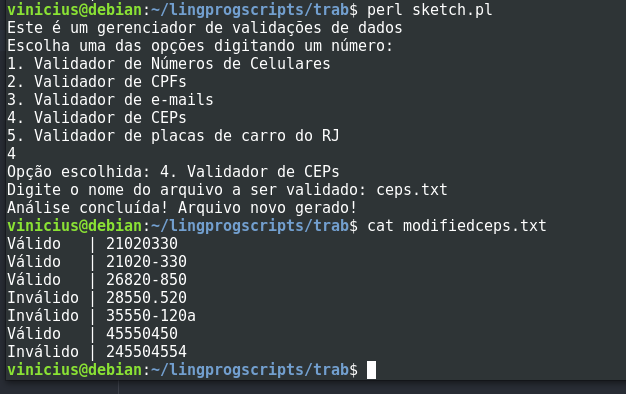
\includegraphics[scale=1]{cep.png}


Na imagem há um exemplo de execução da opção 4., também é mostrada na imagem o conteúdo do arquivo novo. O arquivo ceps.txt usado está incluso na pasta do trabalho.

 No caso de ser chamada a opção do Validador de CPFs, o usuário é questionado sobre a utilização do algoritmo, sendo feita uma recomendação para que se use esta opção:

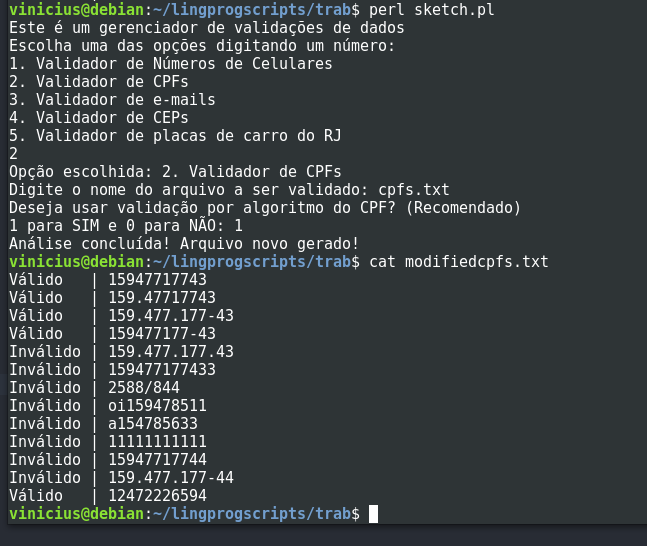
\includegraphics[scale=1]{cpf.png}

Note que, por mais que o penúltimo CPF obedeça à formatação, não foi validado, por não ter passado no teste de soma.

\section{Comentários e Conclusão}

Foram incluídos na pasta do trabalho todos os arquivos de texto usados para os testes das cinco funções. Uma pequena observação: a execução do script nas imagens está com um nome diferente do que foi dado após o término do código, a execução agora, seria evidentemente dada por \textbf{\textit{perl main.pl}}. A opção de não exibir ao usuário diretamente o arquivo criado na tela é uma opção de segurança contra arquivos muito grandes, que poderiam congelar a linha de comando ou atrapalhar o usuário com excesso de informação. Ao longo do projeto a função de números de celular se mostrou bem inconsistente e às vezes pouco confiável, apesar de haver uma complexidade muito grande quando os dados são livres de restrições acredito que a expressão possa ser melhorada com mais testes. Além dessa ressalva o programa se comporta bem e cumpre de forma consistente o seu propósito. Para análise semântica e variações das regex, usei intensivamente o site \textit{https://regex101.com/}.


\end{document}
